\chapter{发动机试验台架}
\section{实验台架}
本实验台架由发动机,发动机支架,发动机附件和其他测试设备组成,其台架系统示意图如\ref{fig:platformintro}图所示。\par
\begin{figure}[!h]
	\centering
	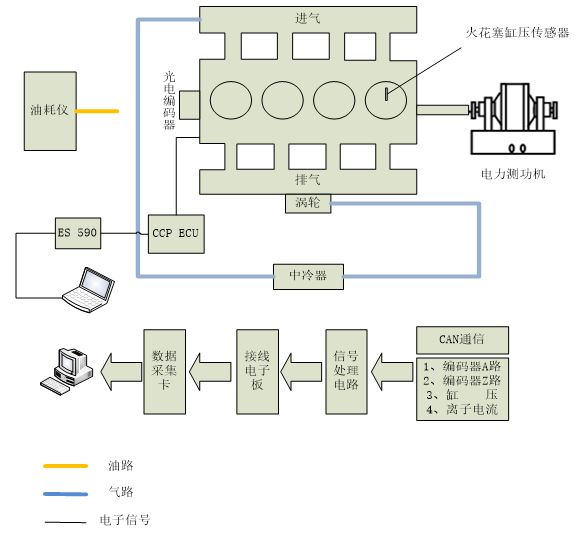
\includegraphics[width=0.85\textwidth]{thesis_figure/platformer_chapter/platformer_intro}
	\caption{台架系统示意图}
	\label{fig:platformintro}
\end{figure}
其中发动机是1.8T涡轮增压多点进气道喷射发动机,电力测功机为凯迈测功机,油耗仪为AVL油耗仪,通过Kistler火花塞式缸压传感器来测量缸压,用光电编码器
来同步信号并确定曲轴上止点位置。通过改造普通的点火线圈将二级线圈高压点和接地点接入离子电流采集电路中来采集离子电流信号。
\subsection{发动机}
发动机实物图如\ref{fig:ecu}所示,该发动机是一台四冲程PFI涡轮增压发动机,缸径为\SI{86}{\mm},行程为\SI{77.4}{\mm},
排量为\SI{1.798}{L},最大功率为\SI{130}{\kW},最大转矩为\SI{230}{\N\m}。
其ECU为联合汽车电子有限公司提供的基于ME788控制系统的ECU,实物图如图\ref{fig:ice}所示。\par
\begin{figure}[!ht]
	\begin{minipage}[h]{0.5\linewidth}
		\centering
		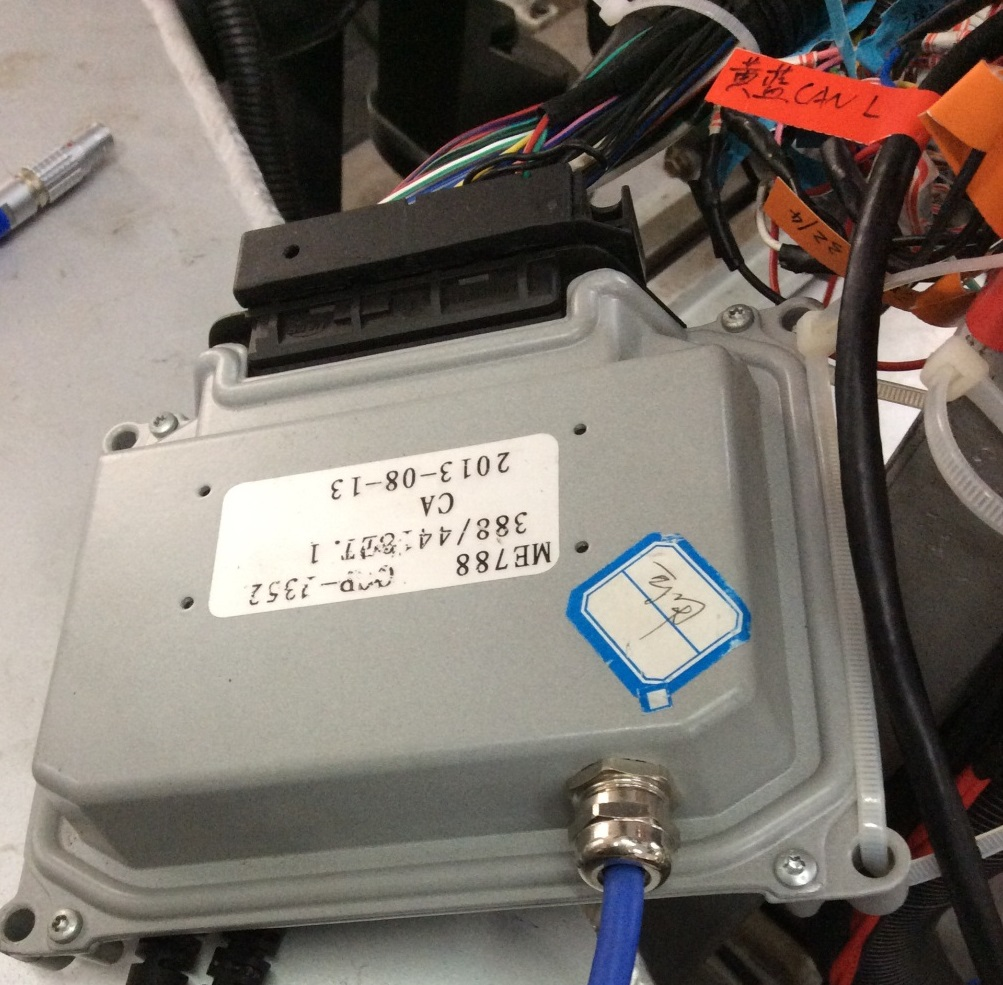
\includegraphics[height=5cm]{thesis_figure/platformer_chapter/ecu}
		\caption{ECU实物图}
		\label{fig:ecu}
	\end{minipage}
	\begin{minipage}[h]{0.5\linewidth}
		\centering
		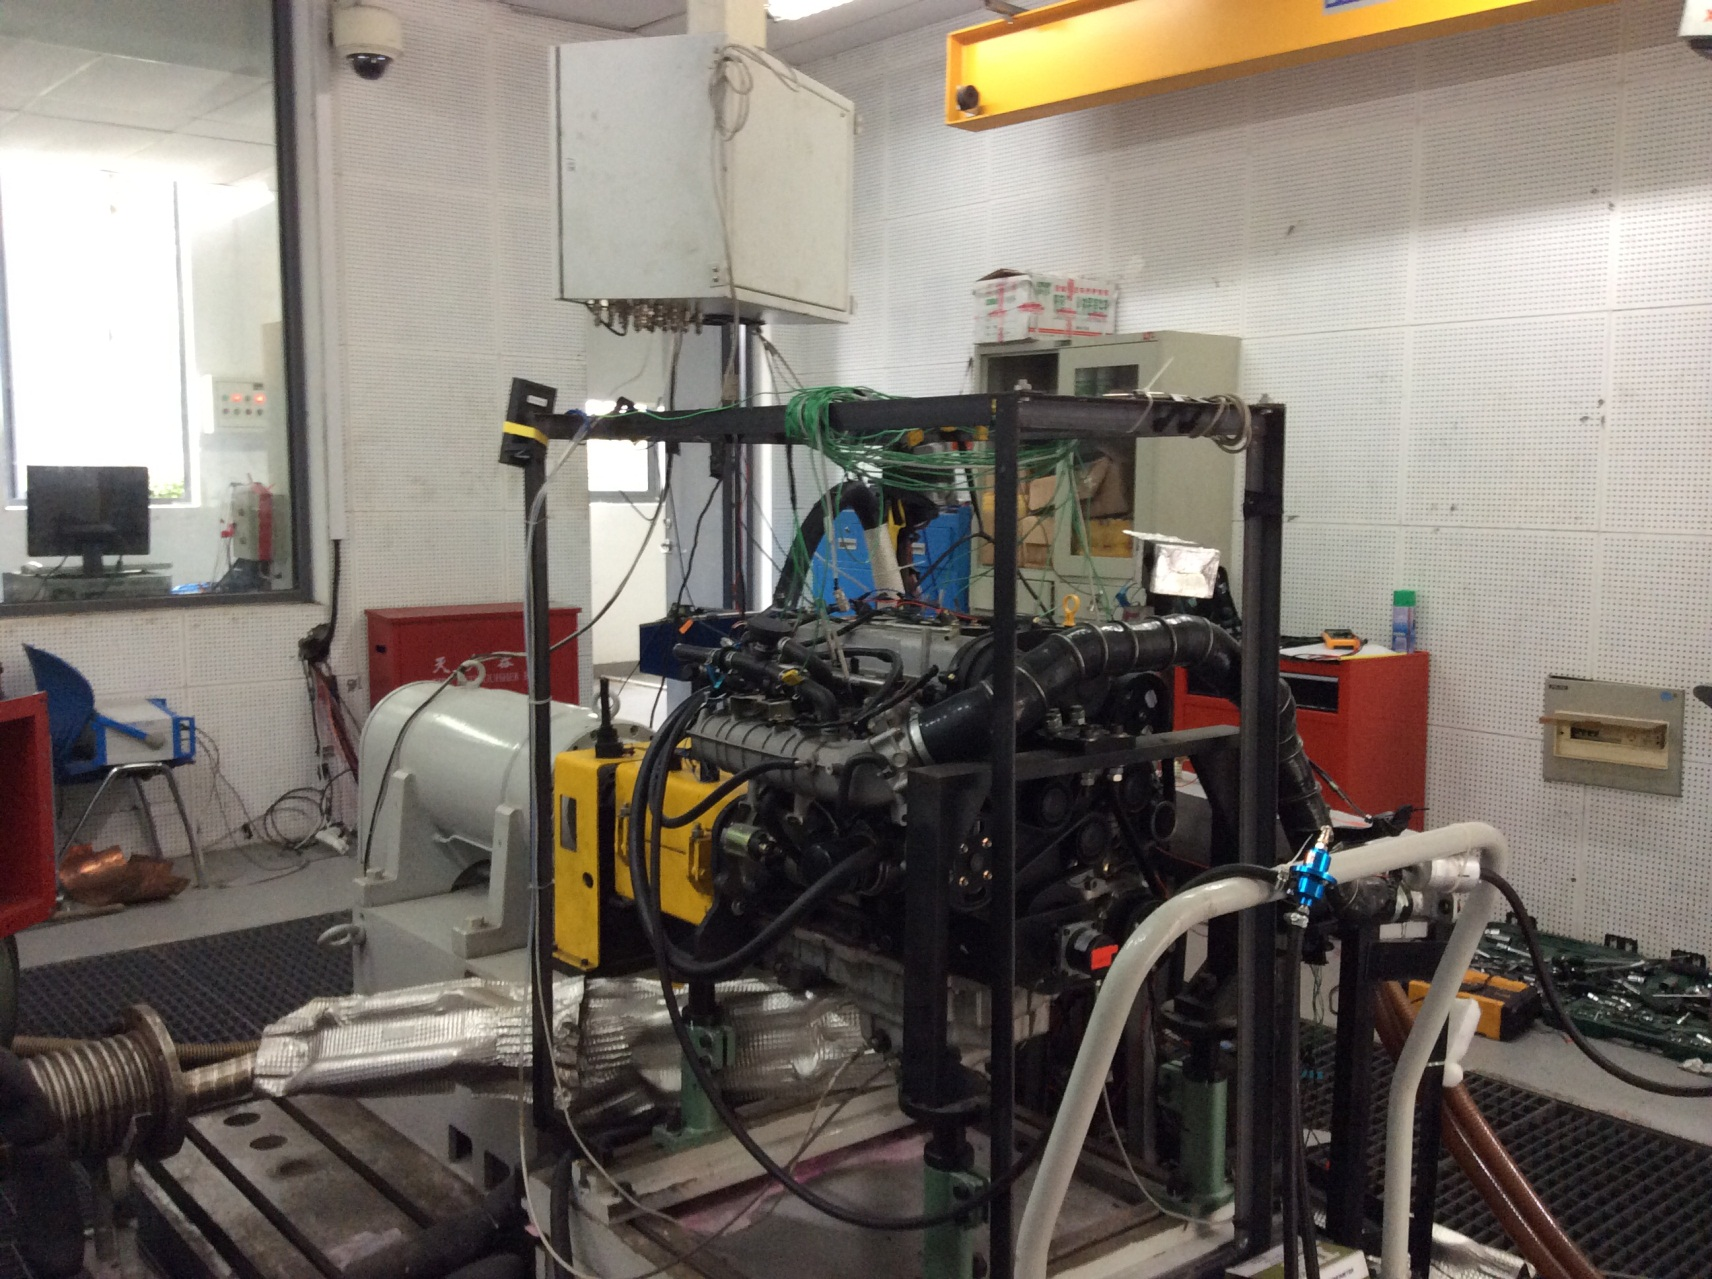
\includegraphics[height=5cm]{thesis_figure/platformer_chapter/ice}
		\caption{发动机实物图}
		\label{fig:ice}
	\end{minipage}
\end{figure}
ECU一端连接发动机线束,另一端通过CAN线连接到上位机。在上位机上安装INCA等软件,通过INCA等软件将该ECU的数据显示并保存出来,用MDA对保存的数据进行简单的数据分析。\par
除此之外,发动机靠近测功机的缸内安装缸压传感器,缸压传感器通过采集卡将数据保存到上位机中。由此,发动机的各项参数可以分别通过ECU和采集卡分别保存到上位机中,通过
采集频率的设定和算法的开发保证分别采集的数据具有相同的采集频率,以便进行后续处理。
\subsection{测功机}
交流电力测功机是目前市场上最先进的动力加载测试设备,在动力机械低速及高速的加载测功实验中都有非常出色的表现,可靠性较高同时又便于维护。
本次实验采用的交流电力测功机系统来自凯迈(洛阳)机电有限公司,该系统基于变频技术开发,精度和稳定性较高,结构简单便于维护,便于进行自动化操作
,形成了一个系列产品。如图\ref{fig:dlcgj}是测功机安装布线的示意图。
\begin{figure}[htb]
	\centering
	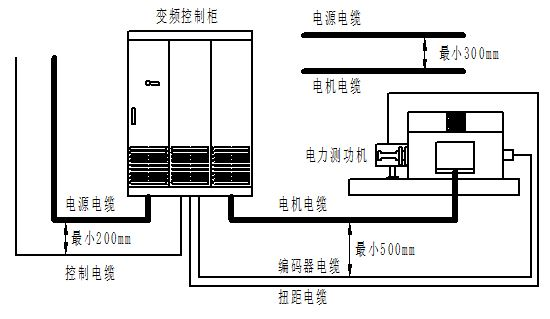
\includegraphics[width=0.75\textwidth]{thesis_figure/platformer_chapter/dlcgj}
	\caption{DCW系列交流电力测功机系统安装布线示意图}
	\label{fig:dlcgj}
\end{figure}
\par 该交流电力测功机主要由三相异步交流电机、可四象限运行的交流调速柜、控制系统、采集系统组成。交流变频调速柜分为整流
单元和逆变单元两部分组成。整流单元可以将380V交流电转换为内部流点,再经过变频成为交流电输出到三相异步电机中。
\begin{figure}[htb]
	\centering
	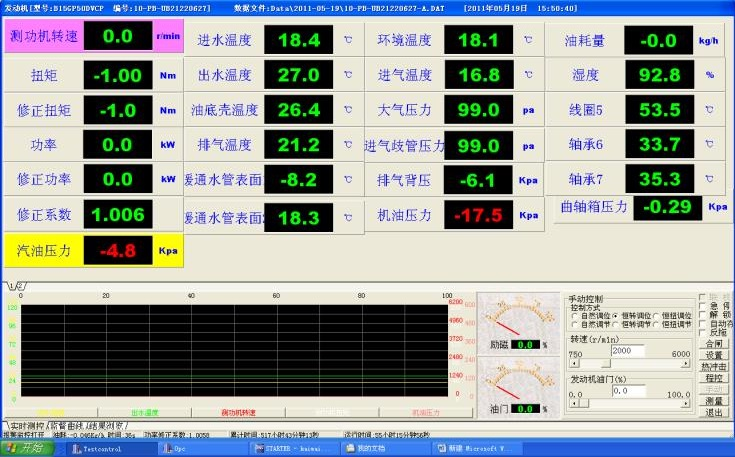
\includegraphics[width=0.75\textwidth]{thesis_figure/platformer_chapter/cgjkzjm}
	\caption{测功机控制界面}
	\label{fig:cgjkzjm}
\end{figure}
\par 测功机的实物图如\ref{fig:dlcgjswt}所示。
测功机通过改变交流电的频率和电压来对测功机的转速进行控制。通过电机四象限转换,将电极交流电转变为工业用电标准的交流电,传到电网,同时可以达到
加载转矩的目的。测功机控制界面如图\ref{fig:cgjkzjm}所示,该界面实时显示台架试验过程中转速、水温、扭矩等状态参数,并具有急停功能。\par
\begin{figure}[htb]
	\centering
	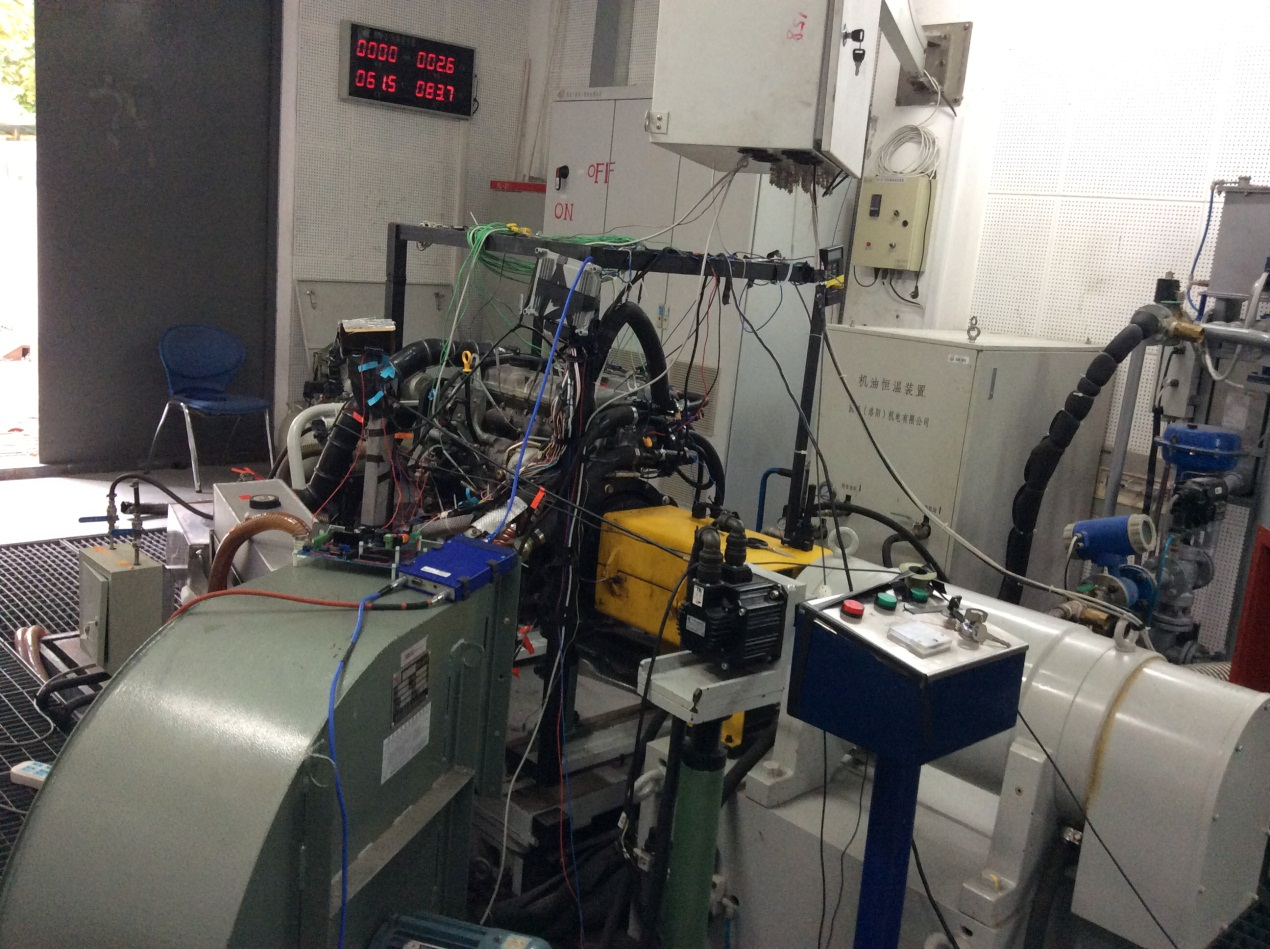
\includegraphics[width=0.75\textwidth]{thesis_figure/platformer_chapter/dlcgjswt}
	\caption{电力测功机实物图}
	\label{fig:dlcgjswt}
\end{figure}
电力测功机的参数如表\ref{tab:dlcgjjtcs}所示,总体来看该测功机性能优秀,适合本实验的进展。
\begin{table}[H] 
 	\centering 
 	\caption{电力测功机具体参数} 
 	\label{tab:dlcgjjtcs} 
 	\begin{tabular}{|c|c|c|} 
 	\hline 
 	测量参数 & 测量范围 & 精度\\\hline 
 	转速 & $0\thicksim10000\si{r/min}$ &$\pm 1\si{r/min}$ \\\hline 
 	扭矩 & $0\thicksim500N\centerdot m$ &$\pm 0.4\%\si{FS}$ \\\hline 
 	燃油消耗 &$0\thicksim100\si{Kg\per h}$ & $\pm 0.12\%\si{FS}$ \\\hline 
 	环境温度 &$0\thicksim50^{\circ}C$ & $\pm 0.5\%\si{FS}$ \\\hline 
 	环境湿度 &$0\thicksim100\%$ & $\pm 2\% RH$ \\\hline 
 	冷却水进温 &$0\thicksim150^{\circ}C$ & $\pm 0.5^{\circ}C$ \\\hline 
 	冷却水出温 &$0\thicksim150^{\circ}C$ & $\pm 0.5^{\circ}C$ \\\hline 
 	机油温度 &$0\thicksim150^{\circ}C$ & $\pm 0.5^{\circ}C$ \\\hline 
 	燃油温度 &$0\thicksim150^{\circ}C$ & $\pm 0.5^{\circ}C$ \\\hline 
 	中冷前温度 &$0\thicksim150^{\circ}C$ & $\pm 0.5^{\circ}C$ \\\hline 
 	中冷后温度 &$0\thicksim250^{\circ}C$ & $\pm 0.5^{\circ}C$ \\\hline 
 	排气温度 &$0\thicksim150^{\circ}C$ & $\pm 0.5^{\circ}C$ \\\hline 
 	机油压力 &$0\thicksim1000\si{KPa}$ & $\pm 0.5\%\si{FS}$ \\\hline 
 	燃油压力 &$0\thicksim1000\si{KPa}$ & $\pm 0.5\%\si{FS}$ \\\hline 
 	进水压力 &$0\thicksim600\si{KPa}$ & $\pm 0.5\%\si{FS}$ \\\hline 
 	出水压力 &$0\thicksim600\si{KPa}$ & $\pm 0.5\%\si{FS}$ \\\hline 
 	曲轴箱压力 &$-20\thicksim20\si{KPa}$ & $\pm 0.25\%\si{FS}$ \\\hline 
 	排气背压 &$0\thicksim50\si{KPa}$ & $\pm 0.5\%\si{FS}$ \\\hline 
 	中冷前压力 &$0\thicksim300\si{KPa}$ & $\pm 0.5\%\si{FS}$ \\\hline 
 	中冷后压力 &$0\thicksim300\si{KPa}$ & $\pm 0.5\%\si{FS}$ \\\hline 
 	大气压力 &$80\thicksim110\si{KPa}$ & $\pm 0.25\%\si{FS}$ \\\hline 
 	\end{tabular} 
\end{table} 
\subsection{发动机附件}
发动机附件包括增压中冷系统、冷却系统、进排气系统等。
增压中冷系统由中冷器、进气、出气、进水、出水、增压压力温度传感器等部分组成。
冷却系统分为水冷和风冷两部分,水冷由外接的冷却循环系统构成。风冷则主要是使用大功
率的风机吹排气管,实现快速降温,使温度在需要范围之内。
进气系统由自制空气滤清器和原机进气管组成,排气系统由原机排气歧管、排气管加上自制一段排气管通往实验室排气系统中,
其中,排气管上装有排气温度传感器。
\section{实验设备及器材}
\subsection{缸压传感器}
缸压传感器采用的是KISTLER提供的6118B型火花塞缸压传感器,具有3mm可换电缆,无需另外打孔即可实现缸压的测量。
它装有世界上最小的压电式高温缸压传感器。安装时,前端与燃烧室内部平齐,固有频率高于100kHz。因此,也可用
于高速发动机和爆震控制测试。其实物图和技术参数见图\ref{fig:gycgq}和表\ref{tab:gycgq}。
\begin{table}[H] 
 	\caption{缸压传感器具体参数} 
 	\label{tab:gycgq} 
 	\centering 
 	\begin{tabular}{|c|c|c|} 
 	\hline 
 	物理量 & 单位& 数值 \\ 
 	\hline 
 	重量 & g& 50\\\hline 
 	压力范围 & bar & $0\thicksim 200$ \\\hline
 	标定区间(在200$^{\circ}C$) &bar & $0\thicksim 150$ \\\hline 
 	过载 & bar & 250 \\\hline 
 	灵敏度(200$^{\circ}C$) & pC/bar & $\thickapprox10$ \\\hline 
 	固有频率 & kHz & $>100$ \\\hline 
 	室温线性度 & \%FSO & $\leq \pm$ 0.5 \\\hline 
 	加速的灵敏度(轴向和径向) & bar/g & $<0.005$ \\\hline 
 	传感器工作温度范围 & $^{\circ}C$ & $-20\thicksim 350$ \\\hline 
 	电缆工作温度范围 & $^{\circ}C$ & $-20 \thicksim 200$ \\\hline 
 	灵敏度变化($200\pm 50^{\circ}C$)&\%& $\leq\pm 1$ \\\hline 
 	短期飘移$\triangle p$ & bar & $\leq \pm 0.6$ \\\hline 
 	$\triangle p_{min}$ & \% & $\leq \pm 3$ \\\hline 
 	$\triangle p_{max}$ & \% & $\leq \pm 1.5$ \\\hline 
 	20$^{\circ}C$时传感器绝缘阻抗 & $\Omega$ & $>1013$ \\\hline 
 	200$^{\circ}C$时传感器绝缘阻抗 & $\Omega$ & $>1011$ \\\hline 
 	火花塞阻抗(1000V,室温下) & $\Omega$& $>100$ \\\hline 
 	绝缘强度 & kV& $<35$ \\\hline 
 	传感器电容 & pF/m& 110\\ 
 	\hline 
 	\end{tabular} 
\end{table}
其还配备了装有数字式双
通道电荷放大器模块的信号调理平台,通过将放大后的气缸压力信号传
给工控机采集卡记录缸内燃烧压力数据。\par
\begin{figure}[htb]
	\begin{minipage}[t]{0.5\linewidth}
		\centering
		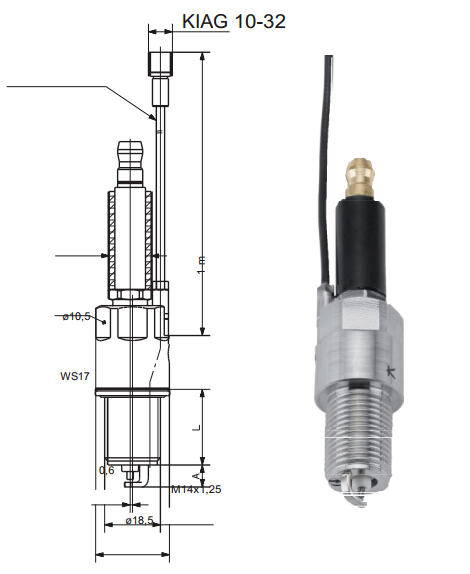
\includegraphics[width=0.8\textwidth]{thesis_figure/platformer_chapter/gycgq}
		\caption{火花塞式缸压传感器}
		\label{fig:gycgq}
	\end{minipage}
	\begin{minipage}[t]{0.5\linewidth}
		\centering
		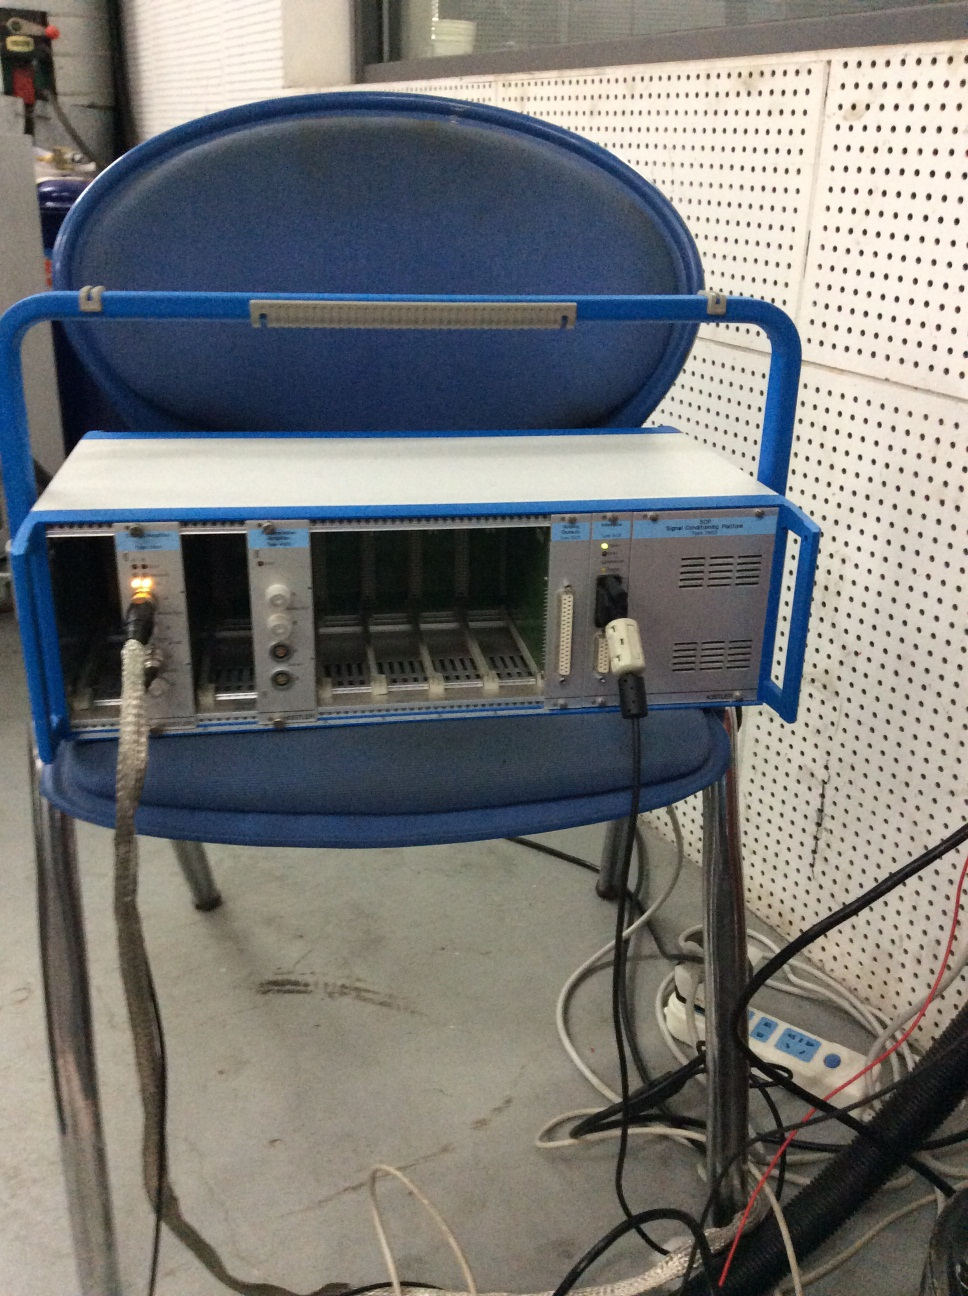
\includegraphics[width=0.8\textwidth]{thesis_figure/platformer_chapter/gycgqdhfdq}
		\caption{缸压传感器电荷放大器}
		\label{fig:gycgqdhfdq}
	\end{minipage}
\end{figure}
这种电荷放大器可以用于实验室通过压电测力仪测量力和扭矩。通过负载作用在压电传感器上产生一个正比例变化的电荷。这
个电荷信号放大器转换成比例的输出电压。电荷放大器的实物图如图\ref{fig:gycgqdhfdq}所示。
\subsection{光电编码器}
发动机正时链条侧曲轴端安装HGAIN公司的F5809型增量式光电编码器,曲轴信号测量范围720 pulse/r,测量精度$0.5^{\circ}CA$,如
图\ref{fig:gdbmq}所示。该编码器内部采用ASIC器件,具有寿命长,可靠性高,信号分辨率高,抗干扰能力较强,信号传输距离较长等优点,为
采集卡提供采样中断保证。其A路与Z路信号用于高速采集系统触发源以及作为后期数据处理的曲轴时刻参考依据。
\begin{figure}[ht]
	\begin{minipage}[H]{0.5\linewidth}
		\centering
		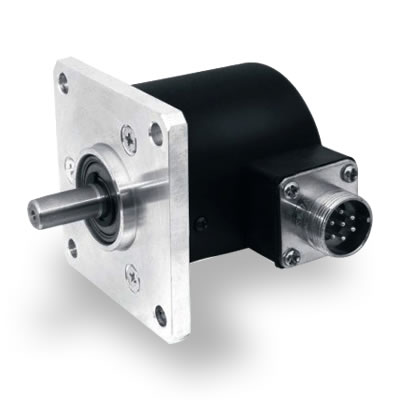
\includegraphics[width=0.8\textwidth]{thesis_figure/platformer_chapter/gdbmq}
		\caption{光电编码器}
		\label{fig:gdbmq}
	\end{minipage}
	\begin{minipage}[H]{0.5\linewidth}
		\centering
		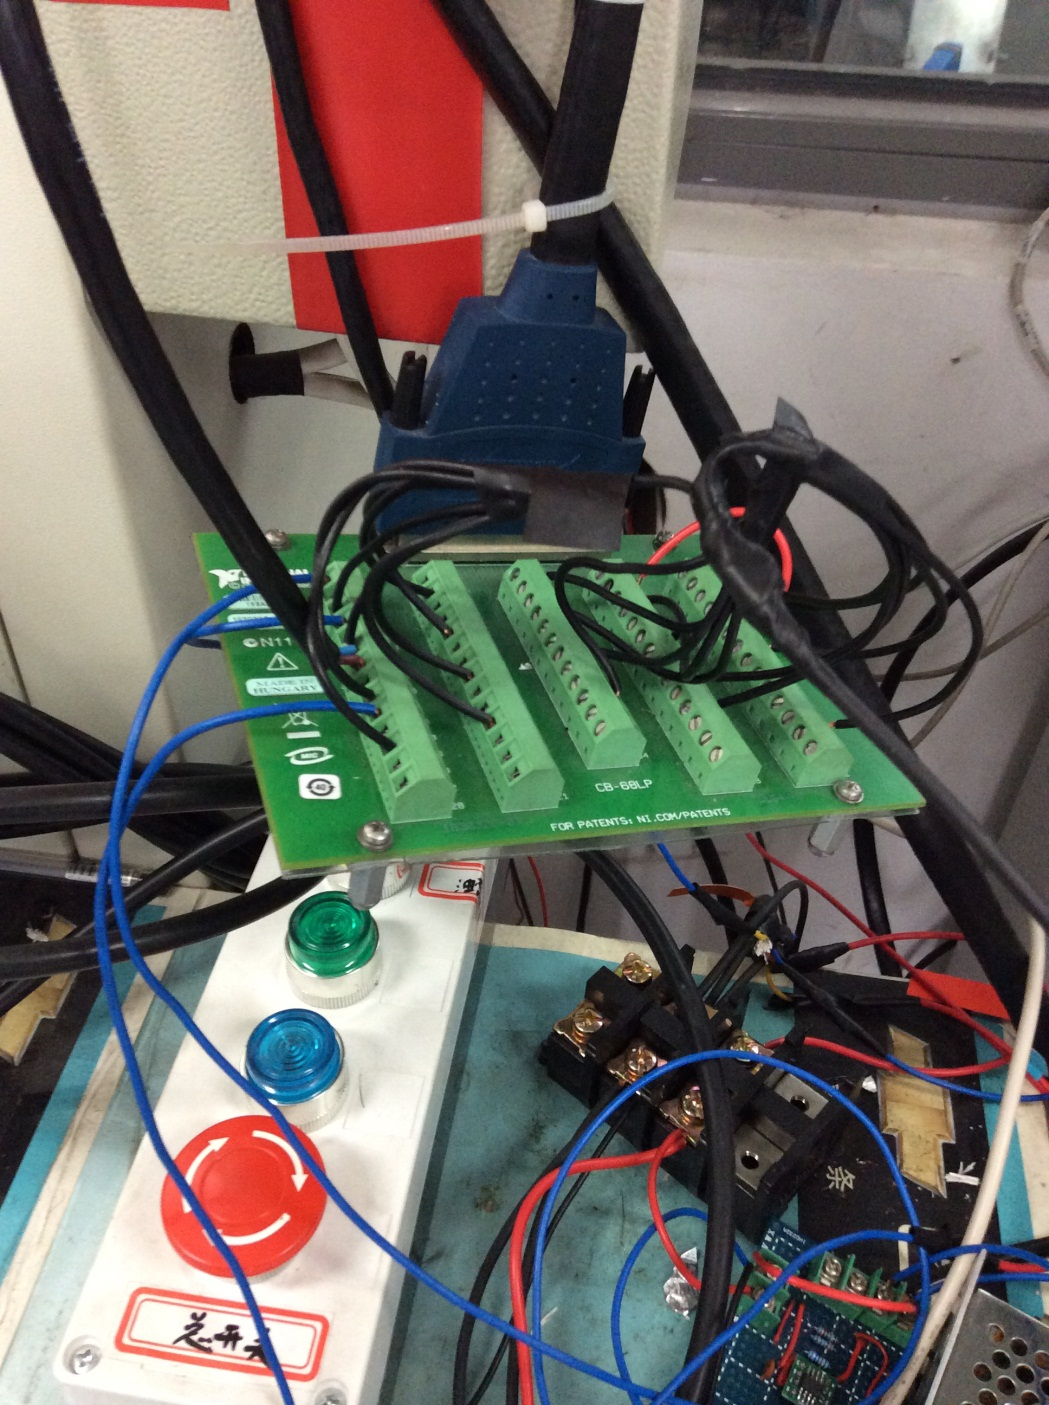
\includegraphics[width=0.8\textwidth]{thesis_figure/platformer_chapter/nicjk}
		\caption{NI公司提供的采集卡}
		\label{fig:nicjk}
	\end{minipage}
\end{figure}
\subsection{采集卡}
数据采集系统可以用来记录发动机运行过程中的各种性能参数。本试验采用NI公司的PCI 6250高速采集卡,其具备16路模拟信号输入,16
位转换精度,多通道采样频率1MHz,单通道模式下1.25MHz,最大采集幅值范围为±10V等强大功能。\par 研究离子电流特性需要采集的参数
分为两大类:第一类是缸内燃烧压力信号、离子电流信号及用于判断曲轴相位的A路和Z路信号等信号,这些信号可以表征发动机的性能和排放;
二是发动机转速、发动机负荷、爆震积分值、进气温度、进气压力、冷却水温度以及机油压力等信号,这些信号主要来自ECU的计算,并通过CAN总线传到高速采集卡中采集下来。该采
集卡能够满足以上两类需求。采集卡实物图如图\ref{fig:nicjk}所示,吊在空中是为了隔离干扰。
\subsection{采集程序}
采集程序是由Labview所编写,主要分为手动采集和触发采集两种类型,可通过记录模式进行切换。其中手动采集模式通过点击“开始”进行数据采
集,而触发采集可以设置触发条件,本文设置的是缸压值$>$阀值,采集程序会将超过该阀值的前后一段时间的数据采集下来,图\ref{fig:cjcxjm}是采集程序的界面。
\begin{figure}[htb]
	\centering
	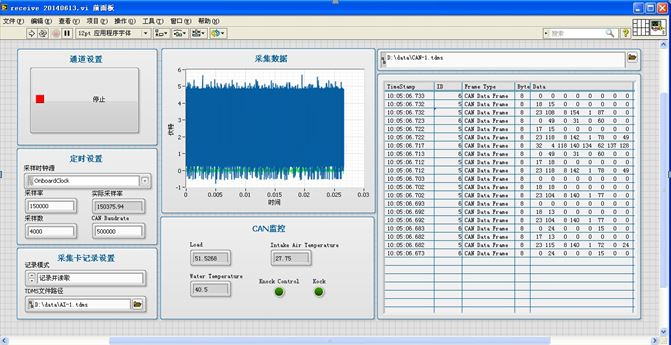
\includegraphics[width=0.85\textwidth,trim=0.25cm 0.5cm 4.5cm 1.25cm,clip]{thesis_figure/platformer_chapter/cjcxjm}
	\caption{采集程序界面}
	\label{fig:cjcxjm}
\end{figure}
\par 该采集程序主要由定时设置,采集卡记录设置,CAN监控,数据实时显示和通道开关几个部分组成。定时设置可以设置采样时钟、采样数、采样率等关键参数;采集卡记录设置
可以设置文件保存的路径,CAN监控可以实时监测采集过程是否有异常,同时也可以通过数据实时显示监控面板来查看数据采集过程是否有异常。





